\documentclass{article}

%%%%%%%%%%%%%%%%%%%%%%%%%
% Packages & Macros
%%%%%%%%%%%%%%%%%%%%%%%%%

% For including graphics
\usepackage{graphicx}

% For title page
\usepackage{datetime}
\newdateformat{monthyeardate}{\monthname[\THEMONTH] \THEYEAR}

% For supporting linking
\usepackage{hyperref}
\hypersetup{colorlinks,urlcolor=blue,linkcolor=blue}

\usepackage{ifthen}

% For table colouring (in command line tables)
\usepackage{colortbl}

%%%%%%%%%%%%%%%%%%%%%%%%%
% Tool-Specific Macros
%%%%%%%%%%%%%%%%%%%%%%%%%
\usepackage{xspace}

\newcommand{\args}[1] {\textit{#1}}
\newcommand{\cmd}[1] {\texttt{#1}}     % Use for command window commands, e.g., \cmd{svn up}
\newcommand{\block}[1] {\textsf{#1}}   % Use for Simulink block names, e.g., \cmd{Subsystem1}
\newcommand{\signal}[1] {\textsf{#1}}   % Use for Simulink block names, e.g., \cmd{Subsystem1}
\newcommand{\ring}[1] {\textsf{#1}} 	 % Use for files names and paths
\newcommand{\keyword}[1] {\texttt{#1}} % Use for keywords of programming languages, e.g., \keyword{while}
\newcommand{\file}[1] {\texttt{#1}} 	 % Use for files names and paths
\newcommand{\param}[1] {\textsf{#1}}   % Use for block parameter names, e.g., \param{BlockType}

% Matlab Products
\newcommand{\matlab}{\textsc{Matlab}\@\xspace}
\newcommand{\Matlab}{\textsc{Matlab}\@\xspace}
\newcommand{\Simulink}{Simulink\@\xspace}
\newcommand{\simulink}{Simulink\@\xspace}
\newcommand{\SDV}{Simulink Design Verifier\@\xspace}
\newcommand{\mpath}{\Matlab search path\@\xspace}

% Block Names (not BlockType)
\newcommand{\ds}{\block{Data Store}\@\xspace}
\newcommand{\DSM}{\block{Data Store Memory}\@\xspace}
\newcommand{\DSR}{\block{Data Store Read}\@\xspace}
\newcommand{\DSW}{\block{Data Store Write}\@\xspace}
\newcommand{\DSRW}{\block{Data Store Read/Write}\@\xspace}
\newcommand{\DSMRW}{\block{Data Store Memory/Read/Write}\@\xspace}

\newcommand{\goto}{\block{Goto}\@\xspace}
\newcommand{\from}{\block{From}\@\xspace}

\newcommand{\inport}{\block{Inport}\@\xspace}
\newcommand{\outport}{\block{Outport}\@\xspace}
\newcommand{\constant}{\block{Constant}\@\xspace}
\newcommand{\ground}{\block{Ground}\@\xspace}
\newcommand{\subsystem}{\block{Subsystem}\@\xspace}

\newcommand{\logic}{\block{Logical Operator}\@\xspace}
\newcommand{\relational}{\block{Relational Operator}\@\xspace}
\newcommand{\ifblk}{\block{If}\@\xspace}
\newcommand{\switch}{\block{Switch}\@\xspace}
\newcommand{\merge}{\block{Merge}\@\xspace}

\newcommand{\docblock}{\block{DocBlock}\@\xspace}

\newcommand{\simfunc}{\block{Simulink Function}\@\xspace}
\newcommand{\simfunccaller}{\block{Function Caller}\@\xspace}

\newcommand{\toworkspace}{\block{To Workspace}\@\xspace}
\newcommand{\fromworkspace}{\block{From Workspace}\@\xspace}

\newcommand{\tofile}{\block{To File}\@\xspace}
\newcommand{\fromfile}{\block{From File}\@\xspace}

\newcommand{\fromspreadsheet}{\block{From Spreadsheet}\@\xspace}

\newcommand{\modelref}{\block{Model Reference}\@\xspace}
\newcommand{\library}{\block{Library}\@\xspace}
\newcommand{\librarylink}{\block{Library Link}\@\xspace}

% Commonly used parameters
\newcommand{\AND}{\param{AND}\@\xspace}
\newcommand{\OR}{\param{OR}\@\xspace}
\newcommand{\NOT}{\param{NOT}\@\xspace}
\newcommand{\NOR}{\param{NOR}\@\xspace}
\newcommand{\NAND}{\param{NAND}\@\xspace}
\newcommand{\XOR}{\param{XOR}\@\xspace}
\newcommand{\NXOR}{\param{NXOR}\@\xspace}

% Common Abbreviations
% Example
\newcommand{\eg}{\textrm{e.g.,}\@\xspace}

% That Is To Say
\newcommand{\ie}{\textrm{i.e.,}\@\xspace}

% And So On
\newcommand{\etc}{\textrm{etc.}\@\xspace}

% And Others
\newcommand{\etal}{\textrm{et al.}\@\xspace}

% With Respect To
\newcommand{\wrt}{\textrm{w.r.t.}\@\xspace}

% Vice Versa
\newcommand{\vrsa}{\textrm{vice versa}\@\xspace}

% Symbols

\usepackage{amssymb}
\newcommand{\checkbox}{\makebox[0pt][l]{$\square$}\raisebox{.15ex}{\hspace{0.1em}$\checkmark$}}%
\newcommand{\uncheckbox}{$\square$~}%


\newcommand{\ToolName}{Simulink Design Documenter\@\xspace}

\newcommand{\menu}[1]{%
	\ifthenelse{\equal{#1}{1}}{Generate Simulink Design Document}{}%
	\ifthenelse{\equal{#1}{2}}{?}{}%
}

\newcommand{\func}[1]{%
	\ifthenelse{\equal{#1}{1}}{GenSDD}{}%
	\ifthenelse{\equal{#1}{2}}{?}{}%
	\ifthenelse{\equal{#1}{3}}{?}{}%
	\ifthenelse{\equal{#1}{4}}{?}{}%
	\ifthenelse{\equal{#1}{5}}{?}{}%
	\ifthenelse{\equal{#1}{6}}{?}{}%
}

\newcommand{\sdd}{Software Design Description\@\xspace}
\newcommand{\demoName}{\cmd{sldemo\_househeat}\@\xspace}

\newcommand{\FCA}{0} 	% Enable/disabled FCA-specific content
%\newcommand{\HowSetPath}{\ifthenelse{\equal{\FCA}{1}}{If it is not, go to \cmd{File~>~Set~Path...}, press \cmd{Add with Subfolders}, and select the \cmd{McMaster\_Tools} folder. Restart \matlab after doing so.}{}}

%%%%%%%%%%%%%%%%%%%%%%%%%
% Document
%%%%%%%%%%%%%%%%%%%%%%%%%

\title{\ToolName}
\date{\monthyeardate\today}

\begin{document}

%%%%%%%%%%%%%%%%%%%%%%%%%%%%%%%%%%%%%%%%%%%%%%%%%%%%%%%%%%%%%%%%%%%
% Title Page
%%%%%%%%%%%%%%%%%%%%%%%%%%%%%%%%%%%%%%%%%%%%%%%%%%%%%%%%%%%%%%%%%%%
\maketitle
\vfill

\begin{figure}
	\centering
	
\includegraphics[]{../../figs/McSCert_Logo.pdf} \\
	McMaster Centre for Software Certification (McSCert)
\end{figure}

\newpage

%%%%%%%%%%%%%%%%%%%%%%%%%%%%%%%%%%%%%%%%%%%%%%%%%%%%%%%%%%%%%%%%%%%
% Table of Contents
%%%%%%%%%%%%%%%%%%%%%%%%%%%%%%%%%%%%%%%%%%%%%%%%%%%%%%%%%%%%%%%%%%%
\tableofcontents
\newpage

%%%%%%%%%%%%%%%%%%%%%%%%%%%%%%%%%%%%%%%%%%%%%%%%%%%%%%%%%%%%%%%%%%%
% Introduction
%%%%%%%%%%%%%%%%%%%%%%%%%%%%%%%%%%%%%%%%%%%%%%%%%%%%%%%%%%%%%%%%%%%
\section{Introduction}

% Briefly, what is the tool?

The purpose of the \ToolName is to facilitate the production of useful \sdd documents for software systems developed with Simulink. While producing documentation is often seen as a tedious task, it is not possible to disregard it since many projects are too large and complex to easily understand without it. The existence of documentation reduces difficulty and time required for software changes and maintenance.


\subsection{More Information}
Further details, as well as additional options and capabilities, can be found in the full guide, located in \href{run:SimulinkDesignDocumenter_FullGuide.pdf}{SimulinkDesignDocumenter\_FullGuide.pdf}.

For more information on the tool and how it can be used in model-based development with \Simulink, please refer to the following papers:

\vspace{1em}
Alexander Schaap, Gordon Marks, Vera Pantelic, Mark Lawford, Gehan Selim, Alan Wassyng, and Lucian Patcas. 2018. \href{https://doi.org/10.1145/3270112.3270115}{``Documenting Simulink Designs of Embedded Systems,"} \textit{Proceedings of the 21st ACM/IEEE International Conference on Model Driven Engineering Languages and Systems (MODELS): Companion Proceedings}, ACM, Copenhagen, Denmark, 47--51.

\vspace{1em}
Vera Pantelic, Alexander Schaap, Alan Wassyng, Victor Bandur, and Mark Lawford. 2019. \href{https://dl.acm.org/doi/abs/10.5220/0007586005030510}{``Something is Rotten in the State of Documenting Simulink Models,"} \textit{Proceedings of the 7th International Conference on Model-Driven Engineering and Software Development}, SciTePress, 503--510.

\subsection{What the \ToolName Provides}

The \ToolName generates a Word document with a title page, clickable table of contents, Changelog,  Document Purpose section, Scope section, design details, a glossary, appendix, and a summary of warnings (if there were any during generation).
The table of contents as well as overall formatting of the document are handled completely automatically, while the title page, Document Purpose, and Scope are also included automatically, though they may be configured or edited.

To provide design details for the system, the \ToolName approaches documentation with the mentality that there will be subsystems within the `main system' which are complex enough to warrant documentation for themselves and as such the \ToolName allows the user to designate subsystems to document and will nest a subsystem's design details within an upper-level system's design details. 
For each system/subsystem being documented the \ToolName will automatically produce 
a picture of the system, a list of subsystems within it, and an Interface section with information about the blocks which are involved in the interface.
Beyond this each system will be documented with 
Purpose, Internal Design, Rationale, and Anticipated Changes sections 
as well as a Requirements Specification section if desired.

\subsection{A Note on Other Software Documentation}
A \sdd document is not the only document that \emph{should} be produced in a project that uses Simulink. Among other documents, Software Requirements Specification documents are also very important to a successful project and they should not be overlooked. However, the \ToolName{} focuses only on \sdd documents.

\newpage	
%%%%%%%%%%%%%%%%%%%%%%%%%%%%%%%%%%%%%%%%%%%%%%%%%%%%%%%%%%%%%%%%%%%
% How to Use the Tool
%%%%%%%%%%%%%%%%%%%%%%%%%%%%%%%%%%%%%%%%%%%%%%%%%%%%%%%%%%%%%%%%%%%
\section{How to Use the Tool}
This section describes what must be done to setup the tool, as well as how to use the tool.

%---------------------------------------
% What needs to be done before the tool can be used? 
% What needs to be done to a model in order for it to work on said model?
%---------------------------------------
\subsection{Prerequisites and Installation}

\begin{enumerate}
	\item Use \matlab/\Simulink R2016b or newer to generate (the model can be saved in earlier versions).
	\item Install the \href{https://github.com/McSCert/Signature}{Signature Tool}.
	\item Ensure Simulink Report Generator is installed (check for it with the \cmd{ver} command in \matlab).
	\item To install the tool,
	\begin{enumerate}
		\item from a \file{.zip} file --- unzip the contents into your desired location. Ensure the unzipped folder and subfolders are present in your \mpath, or add them if they are not present. Run \href{https://www.mathworks.com/help/simulink/ug/registering-customizations.html}{sl\_refresh\_customizations} to refresh the Context Menu. 
		\item from a \file{.mltbx} file --- simply open \Matlab and double-click on the file. Your \mpath should be automatically configured.
		\item from the files only --- add the folders and subfolders to your \mpath. Run \href{https://www.mathworks.com/help/simulink/ug/registering-customizations.html}{sl\_refresh\_customizations} to refresh the Context Menu.
	\end{enumerate}
	\begin{itemize}
		\item \textit{Note:} If running the command ``\cmd{which Interface}'' indicates that the script is not found, then the tool needs to be added to the \mpath.
		For information on adding files to the \mpath, please see the \href{https://www.mathworks.com/help/matlab/matlab_env/add-remove-or-reorder-folders-on-the-search-path.html}{MathWorks documentation}.
	\end{itemize}
	\item Ensure the Simulink-Utility folder is on your \mpath. This is a dependency for the tool to work correctly.
	\item Ensure your model is open (or loaded, for command line use).
\end{enumerate}

%---------------------------------------
% How/when do you access the tool?
%---------------------------------------
\subsection{Getting Started}
The \ToolName can be used via the Simulink Context Menu, which can be viewed by right-clicking in a model.
The following option will be available in the Context Menu (as shown in Figure~\ref{FIG:contextMenu}):
\begin{itemize}
	\item \emph{\menu{1}}
\end{itemize}

\begin{figure}
	\centering
	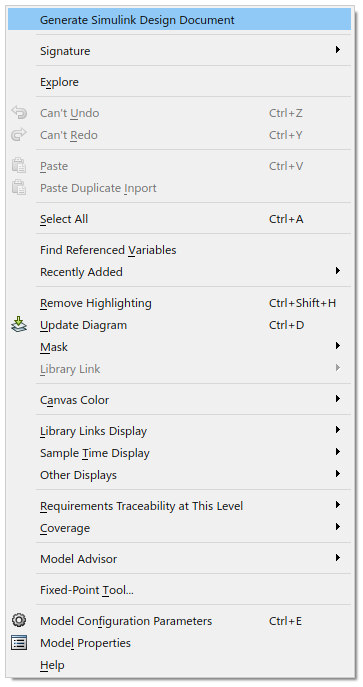
\includegraphics[width=0.6\textwidth]{../../figs/ContextMenu}
	\caption{Simulink Context Menu with tool option visible}
	\label{FIG:contextMenu}
\end{figure}

%---------------------------------------
% What are the main uses of the tool?
%---------------------------------------
\subsection{Functionality}

This section describes the tool functionality when being used from the Simulink Context Menu.

\subsubsection{Report Configuration}
Prior to report generation, the report needs to be configured by the user. Specifically, a configuration file is needed to set up options on how the document will generate (e.g., adding a title image, specifying authors, etc.).
This file must be placed on the \matlab path and named \cmd{<MySystem>\_SDD\_Config.m}. A template configuration file, that also explains the different options available, can be found at \cmd{Report\_Specific\_Files/TopsysName\_SDD\_Config.m}. This template can be duplicated, renamed according to the system you wish to document, and altered to fit one's needs. In particular, users are urged to choose a list of subsystems in \cmd{MySystem} to document, and set the \emph{subsystemList} variable with this information.

\subsubsection{Report Content}
\label{SEC:ReportContent}
Next, the user must add \block{DocBlock}s to the system being documented as well as those subsystems listed by the subsystemList variable. The four mandatory \block{DocBlock}s are: ``Purpose'', ``Internal Design'', ``Rationale'', and ``Anticipated Changes''. The purpose of these blocks is to store useful information describing the system, in order to help others to understand and work with the model. Therefore, after adding these four blocks, the user should open them and populate them with information:

	\begin{itemize}
		\item The \block{Purpose DocBlock} should describe the purpose of the system.
		\item The \block{Internal Design DocBlock} should describe how the system works to accomplish the purpose.
		\item The \block{Rationale DocBlock} should describe why certain design decisions were made.
		\item The \block{Anticipated Changes DocBlock} should describe expected changes to the system (such as from changes in project scope or requirements).
	\end{itemize}

To assist the user, the \keyword{SDD Blocks} block library provides these blocks. This library contains both mandatory and other optional \block{DocBlock}s. The mandatory blocks are shown in Figure~\ref{FIG:libraryBrowser}). The default contents of the blocks briefly explains what content should be stored in them.

Note, one may use ordinary \block{DocBlock}s, however they must have the specific names required by the tool, as given in the \keyword{SDD Blocks} library.

\begin{figure}
	\centering
	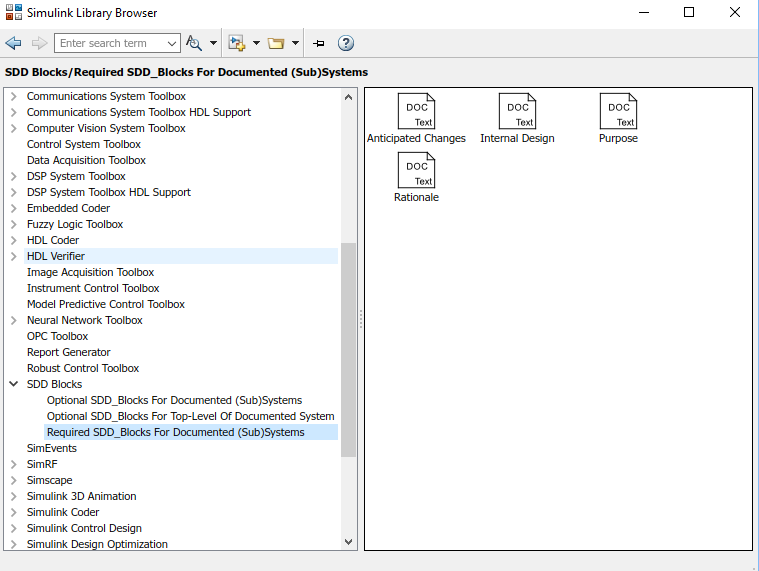
\includegraphics[width=\textwidth]{../../figs/LibraryBrowser}
	\caption{\keyword{SDD Blocks} library in the library browser, showing which \block{DocBlock}s are required for each system/subsystem being documented}
	\label{FIG:libraryBrowser}
\end{figure}

If a user attempts to generate without creating the configuration file or adding the \block{DocBlock}s, the generated document will include warnings at the end of the document which explain what to do (as shown in Figure~\ref{FIG:summaryOfWarnings}):

\begin{figure}
	\centering
	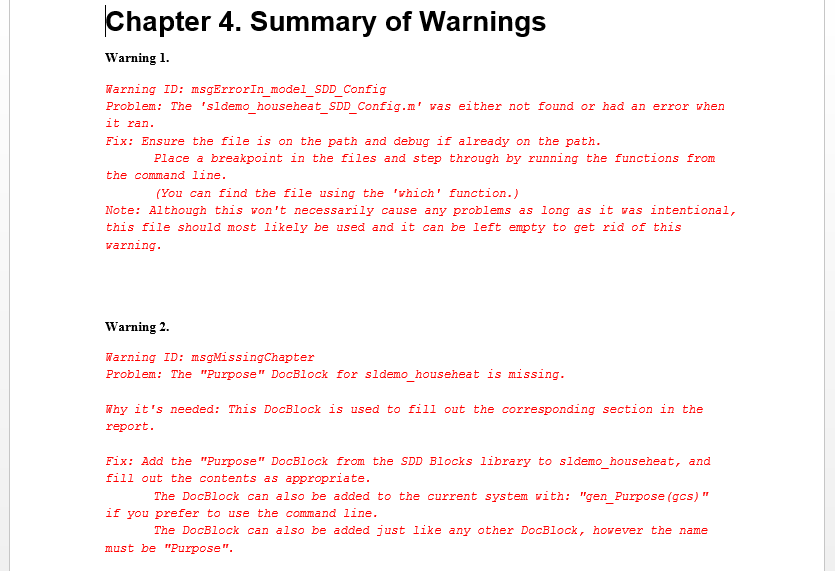
\includegraphics[width=0.8\textwidth]{../../figs/SummaryOfWarnings}
	\caption{Summary of Warnings section in a report generated for the \demoName system}
	\label{FIG:summaryOfWarnings}
\end{figure}

\subsubsection{Report Generation}
Finally, to generate the \sdd document, right-click anywhere in the model and then select \cmd{\menu{1}} from the Context Menu. This will begin the generation of a \sdd document. This document will be named \cmd{SDD\_<MySystem>.docx}, and saved in the current folder in \matlab.

%---------------------------------------
% What else does the tool do?
%---------------------------------------
\subsection{Errors and Warnings}
Any errors or warnings during tool use will be visible in the \matlab Command Window or at the bottom of the generated document. Typically, warnings will occur when any of the mandatory \block{DocBlock}s are missing (i.e., Purpose, Internal Design, Rationale, or Anticipated Changes), or if an appropriately named configuration file is not found.

%%%%%%%%%%%%%%%%%%%%%%%%%%%%%%%%%%%%%%%%%%%%%%%%%%%%%%%%%%%%%%%%%%%
% Example
%%%%%%%%%%%%%%%%%%%%%%%%%%%%%%%%%%%%%%%%%%%%%%%%%%%%%%%%%%%%%%%%%%%
\section{Example}

This section provides simple demonstration of the \ToolName. For a more in depth example, please see the full guide, located in \cmd{SimulinkDesignDocumenter\_FullGuide/FullGuide.pdf}.

Let us create documentation for the top-level of the \demoName model, which is built into \matlab. It is shown in Figure~\ref{FIG:demoModel}.

\begin{figure}
	\centering
	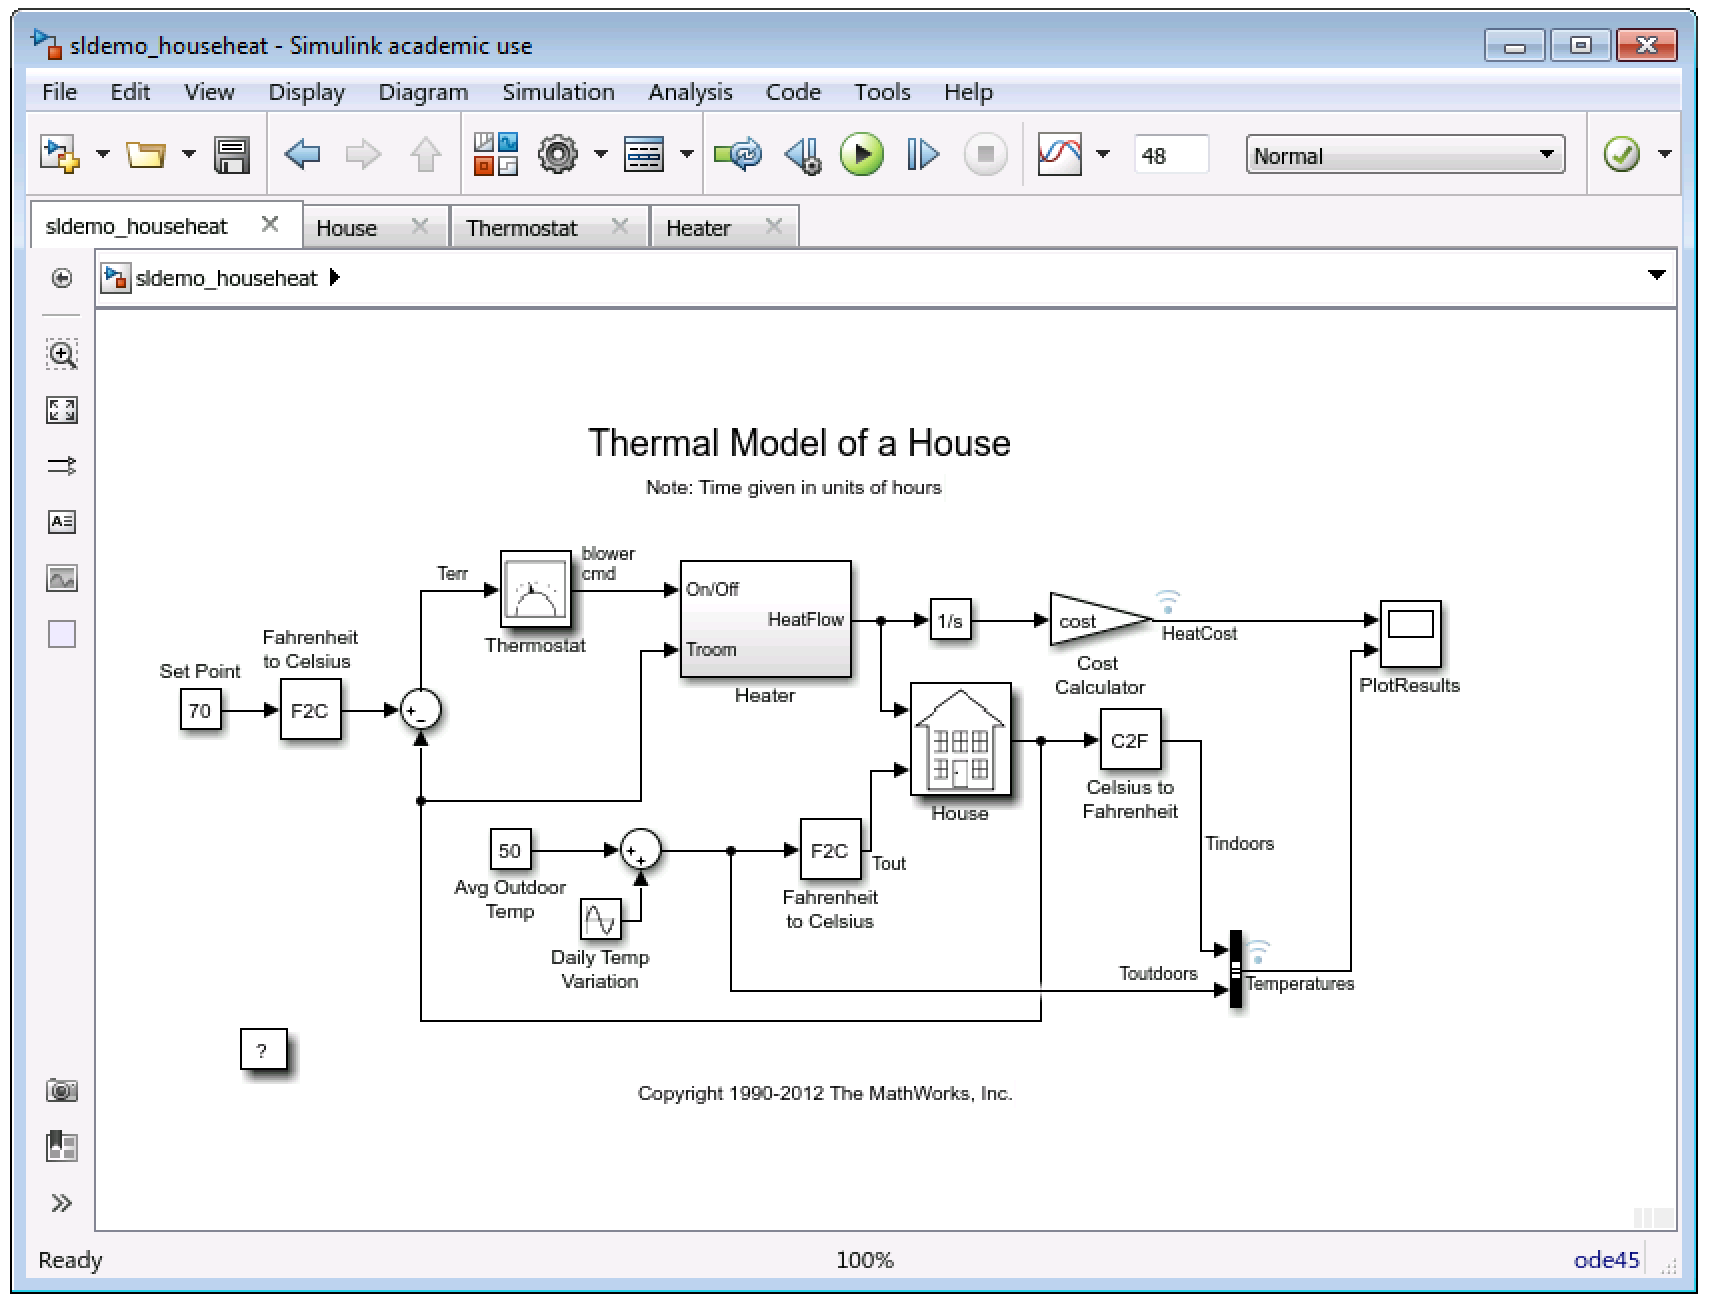
\includegraphics[width=0.9\textwidth]{../../figs/Demo1}
	\caption{The \demoName system}
	\label{FIG:demoModel}
\end{figure}

The following steps will demonstrate the creation of a simple \sdd document.

\begin{enumerate}
	\item Use the command \demoName in the Simulink command window to open the
example model
	\item Create a file on the \matlab path called ``\verb|sldemo_househeat_SDD_Config.m|''. Insert the following lines:
	\begin{itemize}
		\item \verb|author = `John Smith';|
		\item \verb|subsystemList = {};|
	\end{itemize}
	This sets the author name and tells the \ToolName to only generate documentation for the top-level of the system.
	\item Add the four mandatory \block{DocBlock}s from the \keyword{SDD Blocks} block library to the top-level system. For each of the \block{DocBlock}s, write meaningful content, as described in Section~\ref{SEC:ReportContent}.
	\item Save each \block{DocBlock} before closing them, and then save the model as well.
	\item From the top-level system, right-click to access the Simulink Context Menu and select \cmd{\menu{1}}
	\item The \sdd document will automatically open when generation is complete.
\end{enumerate}

%%%%%%%%%%%%%%%%%%%%%%%%%%%%%%%%%%%%%%%%%%%%%%%%%%%%%%%%%%%%%%%%%%%
% Matlab Commands
%%%%%%%%%%%%%%%%%%%%%%%%%%%%%%%%%%%%%%%%%%%%%%%%%%%%%%%%%%%%%%%%%%%
\clearpage
\section{Matlab Commands}

The tool can also be used via the \matlab command line, with the following function(s).

%---------------------------------------
% Command 1
%---------------------------------------
\begin{center}
	\begin{tabular}{| >{\columncolor[gray]{0.9}}l | p{10.5cm} |} \hline
		Function 		& \cmd{\func{1}} \\ \hline
		Syntax			& \cmd{\func{1}}(\args{topsys}) \\ \hline
		Description		& Generate the \sdd document for \args{topsys}. \\ \hline
		Inputs				& \args{topsys}: Name of the system to generate the documentation for.
		It should be a specific subsystem name. \\[.5em]
		Outputs				& N/A \\ \hline	
	\end{tabular}
\end{center}

%%---------------------------------------
%% Command 2
%%---------------------------------------
%\begin{center}
%	\begin{tabular}{| >{\columncolor[gray]{0.9}}l | p{10.5cm} |} \hline
%		Function 		& \\ \hline
%		Syntax			& \\ \hline
%		Description		& \\ \hline
%		Inputs			& \\ \hline	
%		Outputs 		& \\ \hline	
%	\end{tabular}
%\end{center}

\end{document}